Crear la siguiente configuración de red y utilizar RIP en las
máquinas uml

Comprobar las tablas de rutas y los mensajes intercambiados

  \begin{figure}[h]
    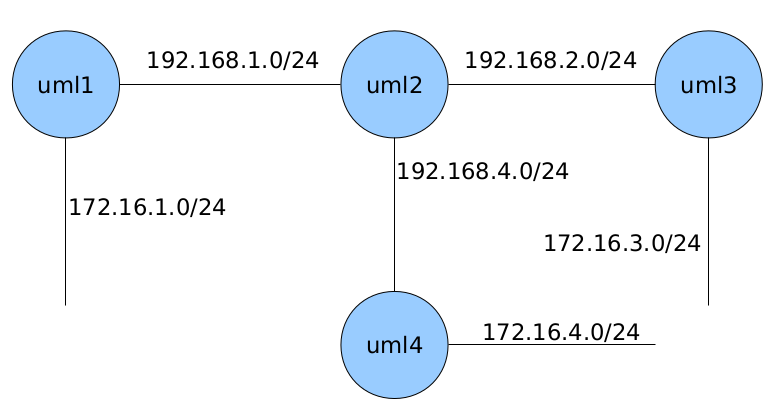
\includegraphics[width=10cm]{ripv1.png}
    \centering
  \end{figure}

  \begin{minted}{bash}
    # net.conf
    defsw br12 uml1.1 uml2.0
    defsw net1 uml1.0
    defsw br23 uml2.1 uml3.1
    defsw br24 uml2.2 uml4.1
    defsw net4 uml4.0
    defsw net3 uml3.0
  \end{minted}

  \begin{minted}{bash}
    # En cuanto se inician las UML, editar el fichero /etc/quagga/daemons la línea
    ripngd=no
    # Por
    ripngd=yes
    # A continuación restart del servicio
    systemctl restart quagga
    # Verificar que se ospfd está corriendo
    systemctl status quagga
\end{minted}

  \begin{minted}{lexer.py:IOSLexer -x}
    ! UML1 (zebra.conf)
    con[figure] t[erminal]
    int[erface] eth0
    ipv6 address 2001:db8:1::1/64
    no s[hutdown]
    q[uit]
    int[erface] eth0
    no s[hutdown]
    q[uit]
    ipv6 f[orwarding]
    w[rite]
  \end{minted}

  \begin{minted}{lexer.py:IOSLexer -x}
    ! UML2 (zebra.conf)
    int[erface] eth0
    no s[hutdown]
    q[uit]
    int[erface] eth1
    no s[hutdown]
    q[uit]
    int[erface] eth2
    no s[hutdown]
    q[uit]
  \end{minted}

  \begin{minted}{lexer.py:IOSLexer -x}
    ! UML3 (zebra.conf)
    con[figure] t[erminal]
    int[erface] eth0
    ipv6 address 2001:db8:3::1/64
    no s[hutdown]
    q[uit]
    int[erface] eth1
    no s[hutdown]
    q[uit]
    ipv6 f[orwarding]
    w[rite]
  \end{minted}

  \begin{minted}{lexer.py:IOSLexer -x}
    ! UML4 (zebra.conf)
    con[figure] t[erminal]
    int[erface] eth0
    ipv6 address 2001:db8:4::1/64
    no s[hutdown]
    q[uit]
    int[erface] eth1
    no s[hutdown]
    q[uit]
    ipv6 f[orwarding]
    w[rite]
  \end{minted}

  \begin{minted}{lexer.py:IOSLexer -x}
    ! UML1 (ripngd.conf)
    con[figure] t[erminal]
    router ripng
      network fe80::/64
      network eth0
      passive-interface eth0
      passive-interface fe80::/64
      do w[rite]
  \end{minted}

  \begin{minted}{lexer.py:IOSLexer -x}
    ! UML2 (ripngd.conf)
    con[figure] t[erminal]
    router ripng
      network fe80::/64º
      passive-interface fe80::/64
      do w[rite]
  \end{minted}

  \begin{minted}{lexer.py:IOSLexer -x}
    ! UML3 (ripngd.conf)
    con[figure] t[erminal]
    router ripng
      network fe80::/64
      network eth0
      passive-interface eth0
      passive-interface fe80::/64
      do w[rite]
  \end{minted}

  \begin{minted}{lexer.py:IOSLexer -x}
    ! UML4 (ripngd.conf)
    con[figure] t[erminal]
    router ripng
      network fe80::/64
      network eth0
      passive-interface eth0
      passive-interface fe80::/64
      do w[rite]
  \end{minted}

  Pruebas:
  \begin{minted}{lexer.py:IOSLexer -x}
    sh[ow] ipv6 rip
    sh[ow] ipv6 route
  \end{minted}